\documentclass{sig-alternate}
\usepackage{amsmath,amsfonts}
\usepackage{multirow}

\begin{document}

\title{Learning to Assess the Cognitive Capacity of Human Partners}

\numberofauthors{1} 

\author{
%
\alignauthor
Anonymous Authors\\
        \affaddr{Department}\\
        \affaddr{University}\\
        \affaddr{City}\\
        \email{anonymous@example.com}
%\alignauthor
%Matthew Atkins\\
%       \affaddr{Oklahoma State University}\\
%       \affaddr{Robotics Cognition Laboratory}\\
%       \affaddr{Stillwater, Oklahoma 74077}\\
%       \email{matthew.atkins@okstate.edu}
%% 2nd. author
%\alignauthor
%S. M. Al Mahi\\
%       \affaddr{Oklahoma State University}\\
%       \affaddr{Robotics Cognition Laboratory}\\
%       \affaddr{Stillwater, Oklahoma 74077}\\
%       \email{smahi@okstate.edu}
%% 3rd. author
%\alignauthor Christopher Crick\\
%       \affaddr{Oklahoma State University}\\
%       \affaddr{Robotics Cognition Laboratory}\\
%       \affaddr{Stillwater, Oklahoma 74077}\\
%       \email{chriscrick@cs.okstate.edu}
}

\maketitle
\begin{abstract} 
We present a robot that learns to recognize the indications that a
complex, rapidly-evolving task has exceeded the cognitive capacity of
a human partner to provide helpful direction.  The robot learns to
associate human directions and task quality metrics in the context of
a well-understood task, in this case, the navigation of a maze.  The
robot is then able to use this learned model to evaluate the behavior
of a human partner in a task which it does not understand and cannot
execute without human instruction.  Even though the context of the new
task is beyond the robot's comprehension, it can accurately assess
whether it is being given trustworthy directions from an increasingly
frazzled human partner.
\end{abstract}

%\category{I.2.9}{Robotics}{Human Assistance}{Multiple Robots}

%\terms{Cognitive Limitation, Trust, Mobile Robot}

\keywords{User modeling and awareness, teamwork and group dynamics,
  robot behavior design, quantitative field study, learning about the
  environment}

\section{Introduction}
One of the most challenging obstacles facing human-robot teams is the
inherent communication barrier between the two. Human operators, at
least once they have received training, have some notion concerning
the capacities of their mechanized partners, but the ability of robots
to assess the limitations of humans has not received adequate
attention. Research in this area often focuses on attempting to
observe human behavior and predict what action or actions to perform
in the future; this renders such systems incapable of making
instantaneous or reactive decisions. In contrast, systems which are
capable of making split-second decisions, such as the lane drift
detection found in some high-end cars, make no inference concerning
the user's abilites or frame of mind; they are reacting to a
well-understood world state without consulting their human
partners. This is not true interaction; the robot is learning to work
\textit{around} the user instead of with them.  Human assistance
should enable complex multi-robot tasks where the robots themselves
are unable to assess their environment fully, but this lays a heavy
burden on the operator in a dynamic, dangerous, rapidly-changing
environment with many cognitive demands.  Fundamentally, human
operators and robots each have complementary capabilities and
limitations, and they must each be aware of the abilities of the
other.  Discovering the cognitive capacity of human operators in
human-robot teams is essential \cite{Malchus:2013:REC:2447556.2447632}.
Our research allows robots to form models of human behavior during
well-understood tasks, and then apply these learned models during
unknown tasks.  We show that these models allow the robot to make an
effective determination of the cognitive capacity of a human partner,
even when the robot cannot directly assess the task it is being asked
to perform.  In this way, a robot team member should be able to fall
back into a safe autonomous mode whenever the task demands begin to
exceed the ability of its human partner to provide effective
direction.

\begin{figure}
\centering
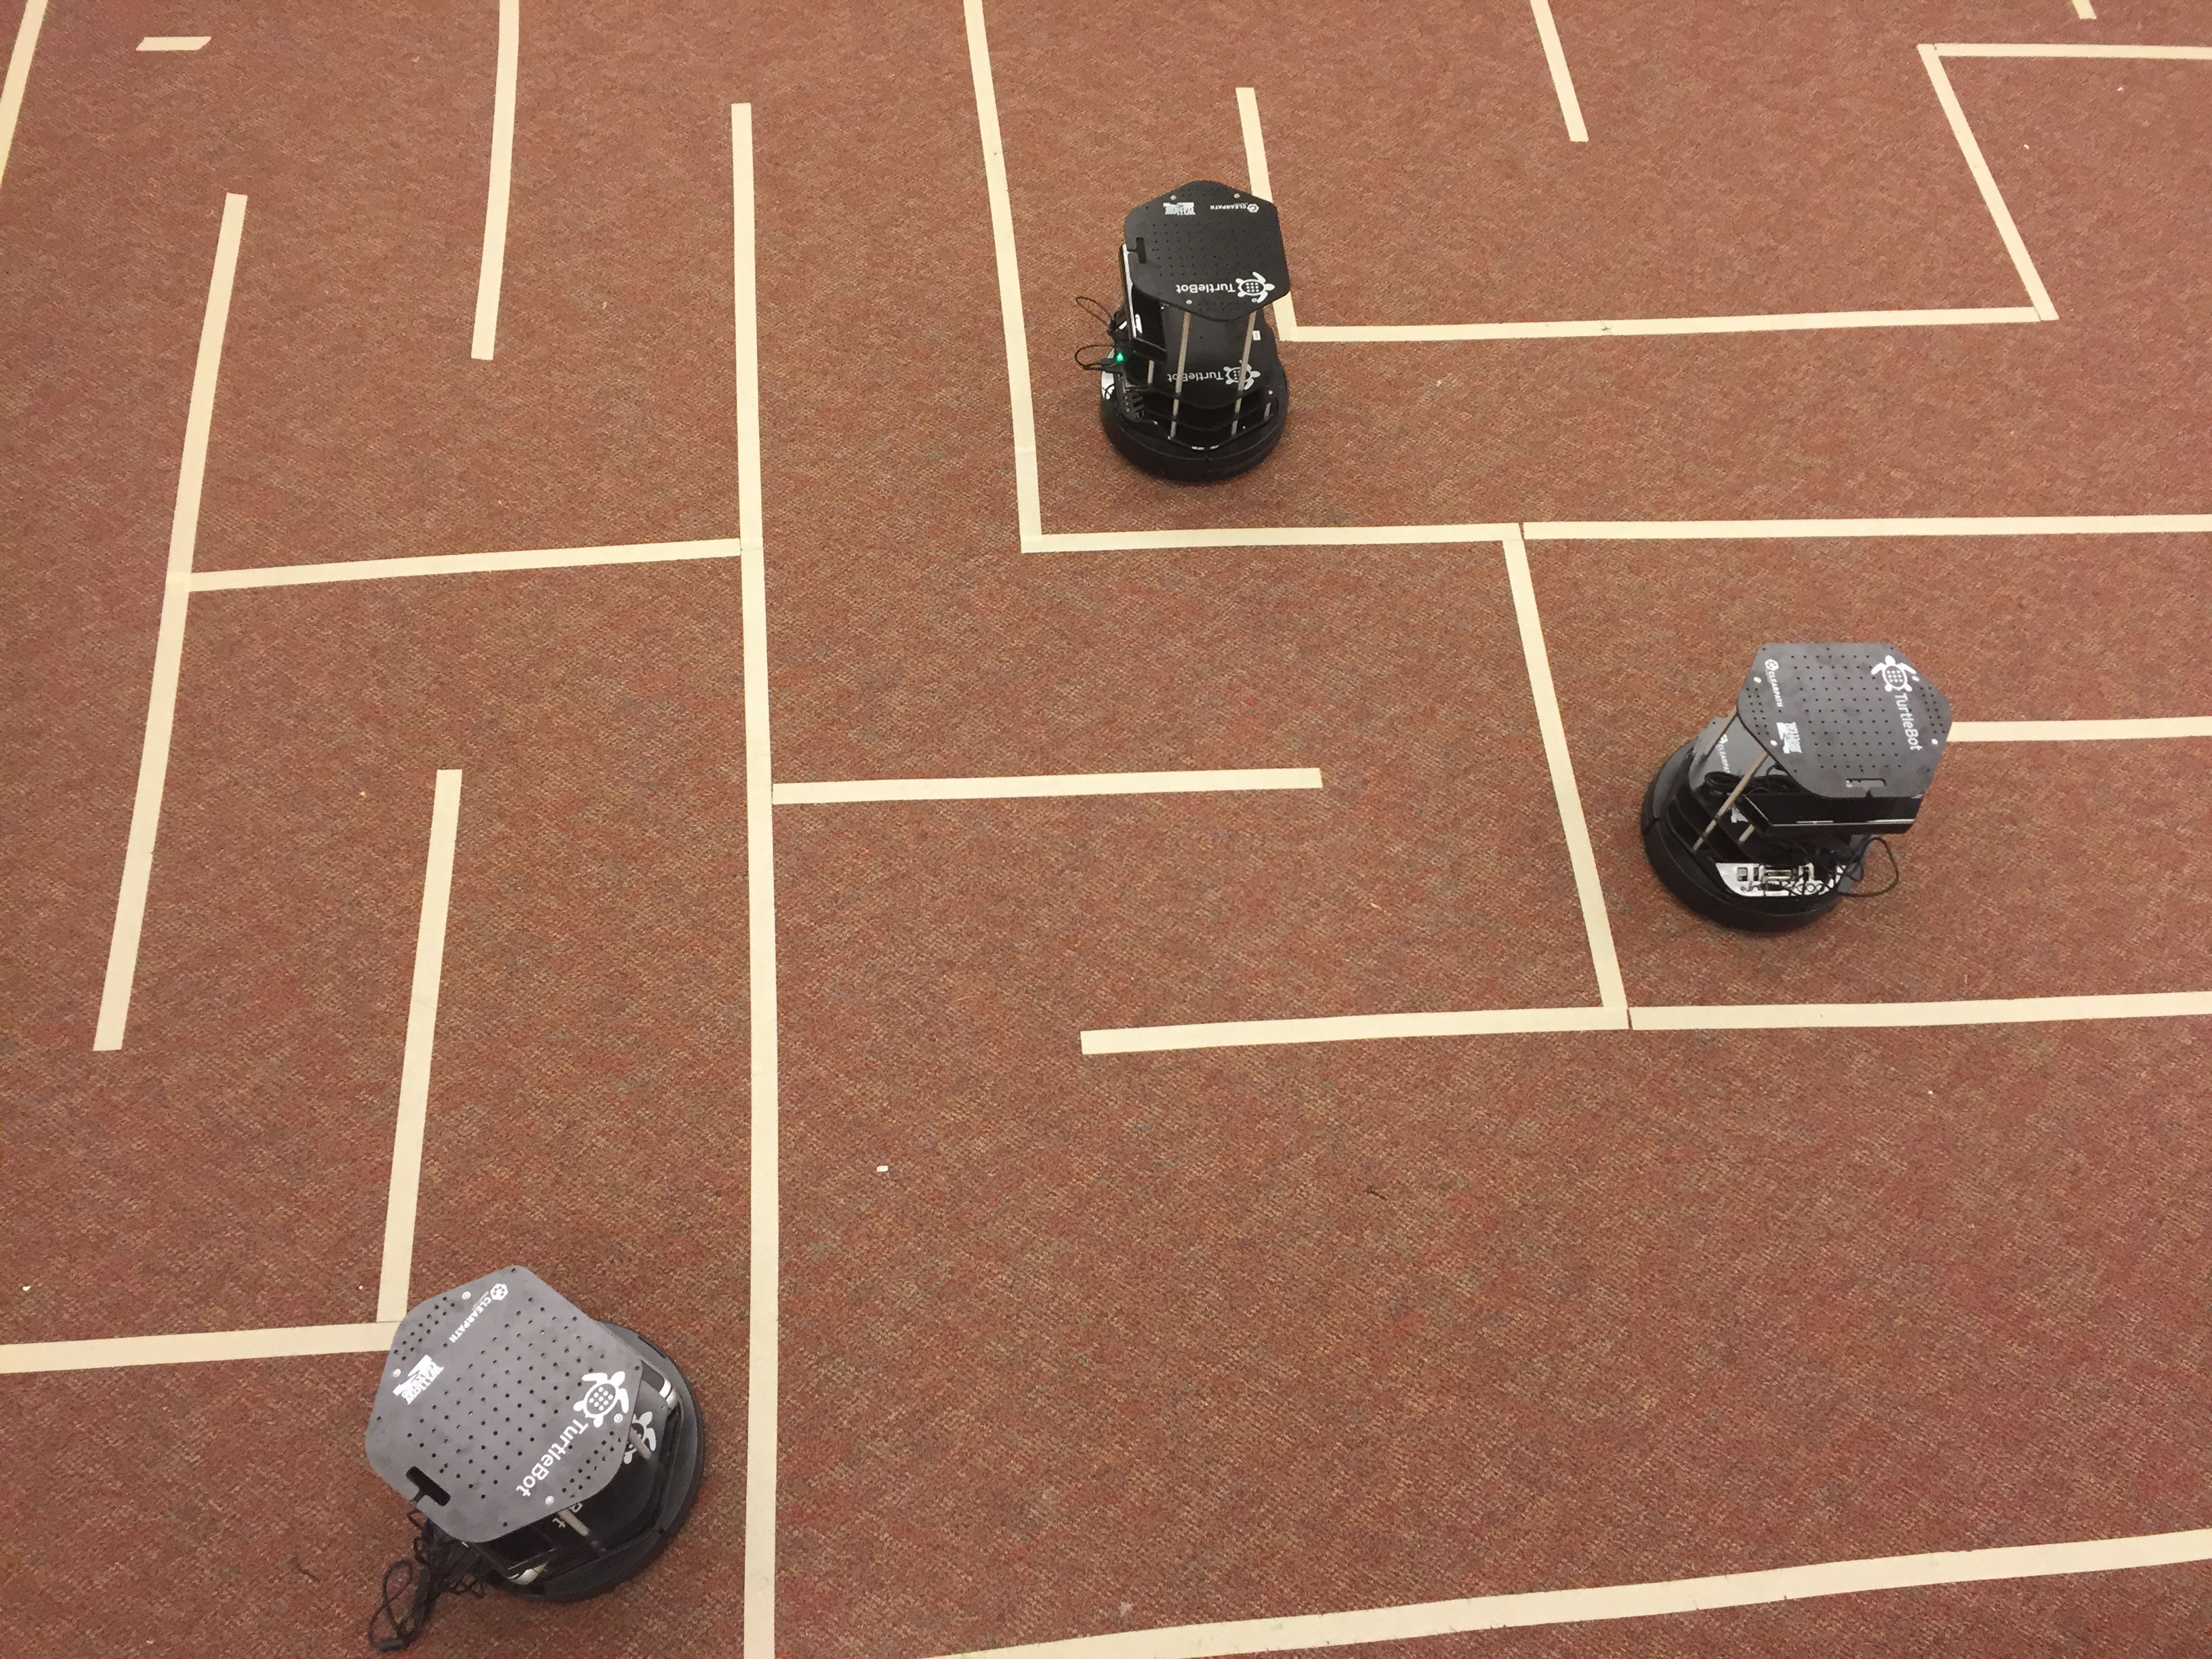
\includegraphics[width=.5\textwidth]{robots-in-maze.jpg}
\caption{Turtlebots navigate a maze while evaluating human task input.}
\label{fig:game_photo}
\end{figure}

Why is teamwork between human and robots so important?  Both have
advantages and limitations. It is easy to understand that a robot with
flawed sensors and actuators may not be able to perform a task, owing
to failure to perceive information about its environment.  But it is
not necessarily the case that improving the sensors and actuators will
have a commensurate effect on the robot's ability to accomplish a task
-- a great many tasks require contextual information far beyond the
current ability of any robot to reason about.  Thus for the forseeable
future, many tasks will require assistance from human teammates, who
are able to integrate data, rely on experience to predict the effects
of actions on world states, and produce effective long-term plans far
better than any current robot.

Human assistance with multiple robots has been demonstrated in
different practical situations. For example, they have been used as
customer assistants in shopping malls \cite{zheng2013supervisory,
  Kanda:2009:AGR:1514095.1514127}, where human operators occasionally
assisted robots. Human-robot teams have assisted each other in museum
tour scenarios \cite{thrun1999minerva} and in warehouse inventory
management \cite{wurman2008coordinating}.  Just as robots, regardless
of their hardware capabilities, do not necessarily perform well
without assistance, humans do not always assist robots as efficiently
as they might, despite their superiority in context sensitivity and
general intelligence.  Several issues arise in this regard
\cite{breazeal2004social}, including obvious problems such as noisy
communication between human operators and robots, accidental damage to
robot sensors and so on.

In this paper, we focus on one problem which can cause difficulties in
a human-robot team: the cognitive capacity of the human operator.
Humans often find their ability to function effectively challenged,
due to psychological stress, tiredness, or overwhelming task demands.
A robot's ability to participate constructively in a human-robot team
will benefit immensely from understanding and accommodating this
cognitive stress appropriately.  For example, for the pilot of an
unmanned aircraft, cognitive stress can be the difference between life
and death \cite{crandall2005validating}.  If such a robot can detect
the emergence of cognitive stress in its operator, it can increase its
level of autonomy and reduce its demands on the operator's attention.
Hopefully, such a robot would wait safely for a more opportune moment
or decide to engage in a less cognitively challenging task, rather
than continue to follow the direction of a human who is no longer able
to provide appropriate assistance.

In this paper, we have designed robots that learn the correlations
between quantifiable behavior metrics and the cognitive capabilities
of human operators.  We designed a maze game
(Fig. \ref{fig:game_photo}) where multiple robots are given directions
by a single human operator.  At first, the robots' objective was
simply to complete the maze, a task that they were capable of
executing without human assistance using autonomous path planning.
They were therefore able to determine whether the instructions of
their operators were sound or questionable, and associated these
outcomes with measurements of their operator's behavior.  We observed
the output of the learned cognitive stress model in a different task,
this time with the robots engaged in a coin-collecting game inside the
maze.  Although the robots had no knowledge of the rules or objectives
of the coin-collecting game, and had no ability to sense the game's
context, their learned models enabled them to determine the cognitive
stress of their human partner.  In this way, they were able to
evaluate the trustworthiness of the actions they were being asked to
perform.  The cognitive stress discerned by the robot correlates with
the true stress experienced by the human operators, as quantified by
their self-reporting and by expert evaluation.

\section{Related Work}
In this section, we will briefly discuss work related to cognitive
capacity assessment and human operation of multiple robots.  Several
research projects recently have investigated human cognitive capacity
using different approaches.

Effectively navigating a maze game has been demonstrated in literature
\cite{crick2011human}.  This research showed that robots learn more
effectively from human operators if the learning took place in the
context of features that the robot can easily understand.
Counterintuitively, restricting the information available to a human
operator led to better demonstrations and more effective learning.  In
this research, we show that similar metrics can be employed by the
robot for the purpose of learning the cognitive threshold of a human
operator.

Recent work \cite{das2013attention,Hoque:2012:ACH:2157689.2157729}
presented a model for assessing a human's attention level, based on
eye contact and gaze detection towards a robot. Based on the perceived
attention level, the robot could generate an appropriate signal to
obtain the attention of a targeted human.  Attention is an important
component of a human agent's cognitive capacity, but in our work, the
robot learns a general behavior model to identify the operator's
cognitive threshold, rather than relying on the specifics of gaze.

Human-robot interactions can be evaluated using fundamental metrics
\cite{olsen2003metrics}. Such metrics relate to the cognitive capacity
of human operators in obvious ways. For example, task effectiveness
(TE) describes how efficiently robots complete a given task under
human direction.  For example, task effectiveness can be measured
using the speed of the robot. In a navigation experiment, it may be
the time taken by the robot to reach the goal.  It could be defined as
the difference between the time taken with and without human
assistance.  Another important metric is neglect tolerance (NT), which
denotes a robot's level of autonomy. In static indoor environments,
simple robots such as Turtlebots can easily engage in autonomous
navigation. Even in complex environments with dynamic obstacles,
clever algorithms \cite{montemerlo2008junior} can enable such vehicles
to navigate autonomously. Thus although it is a very important metric,
we have focused on mostly TE because we think that that is the metric
which can be exploited more consistently across different problems.
Other potentially useful metrics include robot attention demand (RAD),
free time (FT), fan out (FO) and interaction time.  All of these could
conceivably be included as inputs into a learned model such as ours.

Other efforts \cite{goodrich2003seven, olsen2003metrics} have
presented very similar concepts of metrics for improving the
efficiency of human-robot interaction. These principles include
implicit mode switching among user interfaces, using human operators'
natural cues, directly manipulating the world, manipulating the
relationship between the robot and the world, supporting attention
management and so on. Using similar terminology, other work
\cite{crandall2005validating} discovered how neglect time impacts
important properties of human robot teams. They have shown a relation
between the neglect time and the maximum number of robot that a single
human operator can handle.  We leverage this data to inform our
robots' estimation of a human operator's cognitive capacity.

In another social experiment \cite{zheng2013supervisory}, where
autonomous humanoid robots have been deployed to investigate their
social acceptance, a scheduling algorithm has been used to assist the
human operator.  This experiment developed an algorithm that
prioritizes the assitance provided by a human operator for a
particular robot within a multi-robot team. The robot's task was to
make conversation with interested shopping mall customers and to guide
them to particular shelves corresponding to their needs. The shopping
mall map was already known.  Within critical areas inside the shopping
mall environment, the robot needed assistance from humans, for example
in unsafe locations or areas with glass walls that confused the
robots' sensors.  As there were multiple robots, a single operator
could not assist them all simultaneously.  The operator allocator
algorithm therefore picked the robot most likely to encounter a
critical region for assistance. In this work, the operator was assumed
to be able to assist the robot without considering cognitive
capacity. In contrast, we developed a model that enables the robot to
make this determination and then perform the task accordingly.

A large amount of work
\cite{thomaz2006reinforcement,thomaz2008teachable} has investigated
human operators acting as teachers when interacting with a robot, for
example helping a robot in kitchen environment. The human's
demonstrations contribute to the robot's reward functions, using a
modified reinforcement learning method that is based on the
observation that human guidance is able to consider future reward
along with past reward.  The rich context that a human operator
provides and that robots are very poor at reasoning about for
themselves leads to improvement in the robot's learned behaviors.
This observation only holds, however, as long as the human operator
possesses the cognitive capacity to provide good, informative
demonstrations.  Our work allows robots to make this determination for
themselves.

We have mentioned a number of research results that relate to ours in
many ways.  However, most current work does not explore the fact that,
although humans are much more intelligent than robots, they
nevertheless face significant limitations in their ability to assist
their robot partners.  One aspect of these limitations is that a human
operator is vulnerable to task overload and psychological stress.  Our
work focuses particularly on human behavior in the face of this
cognitive stress.  Although engaging human assistance for the purpose
of task learning is valuable, we argue that such a learning task is
more effective if the robot simultaneously has the tools to evaluate
the trustworthiness of the human's direction.

\section{Technical Details}
For our research project, experiments were carried out in two parts:
the Maze Game and the Coin Game experiments. In the first phase, the
robot was run through the maze in order to collect the data needed to
build a model for evaluating the trustworthiness of user input. The
robot is able to do this for the first phase because in the case of
the maze game it understands the problem sufficiently to make such a
judgement; the robot requires no human aid to solve this problem.

\begin{figure}
\centering 
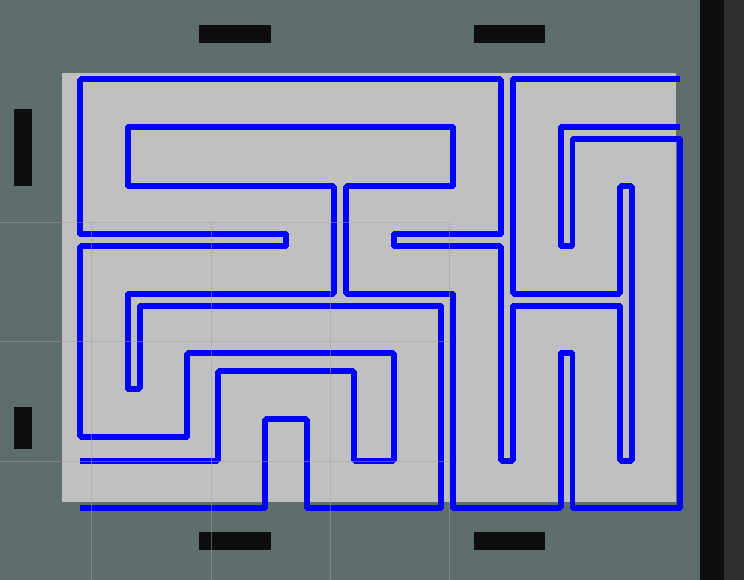
\includegraphics[width=.5\textwidth]{rviz_maze.png} 
\caption{Representation of the path through the maze in RViz.}
\label{fig:rviz_map}
\end{figure}

\begin{figure}
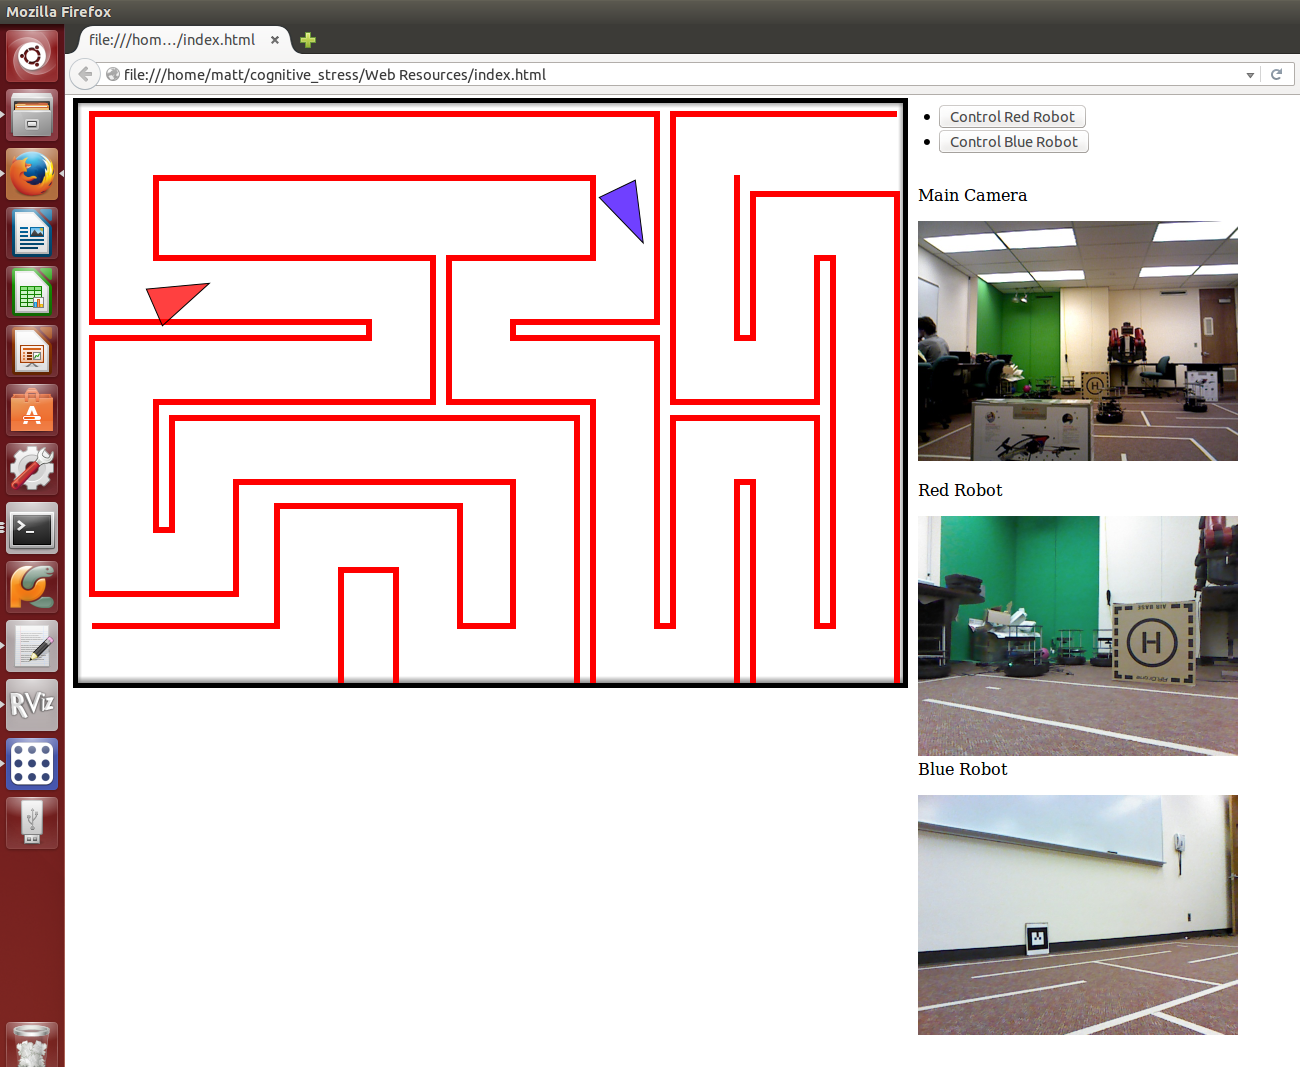
\includegraphics[width=.5\textwidth]{web-controller.png}
\caption{The Rosbridge Web Interface.}
\label{fig:web_interface_img}
\end{figure}

In the Coin Game portion of the project, the robot was placed in a
scenario that shared many similar features with the maze game but with
one crucial difference: the robot's understanding of the problem was
incomplete. While each of the subgoals were individually solvable by
the robot, its model of the overall problem was intentionally
incomplete. For the robot, each subgoal was effectively like solving a
trivial maze in the previous experiment. Both the similarities and
differences between the two experiments were crucial as they allowed
us to test the performance of the previously learned trust model in a
more generalized scenario.

Communication between operators and robots was achieved using the
Robot Operating System (ROS)\cite{quigley2009ros}.  Users sent
navigation goals to the robots using ROS's built-in visualization
tool, Rviz (Fig~\ref{fig:rviz_map}), or by using a web interface
developed for the project, which allowed the experiment to be
conducted remotely (Fig~\ref{fig:web_interface_img}).

\section{Maze Game and Training}
  
\begin{figure}
\centering
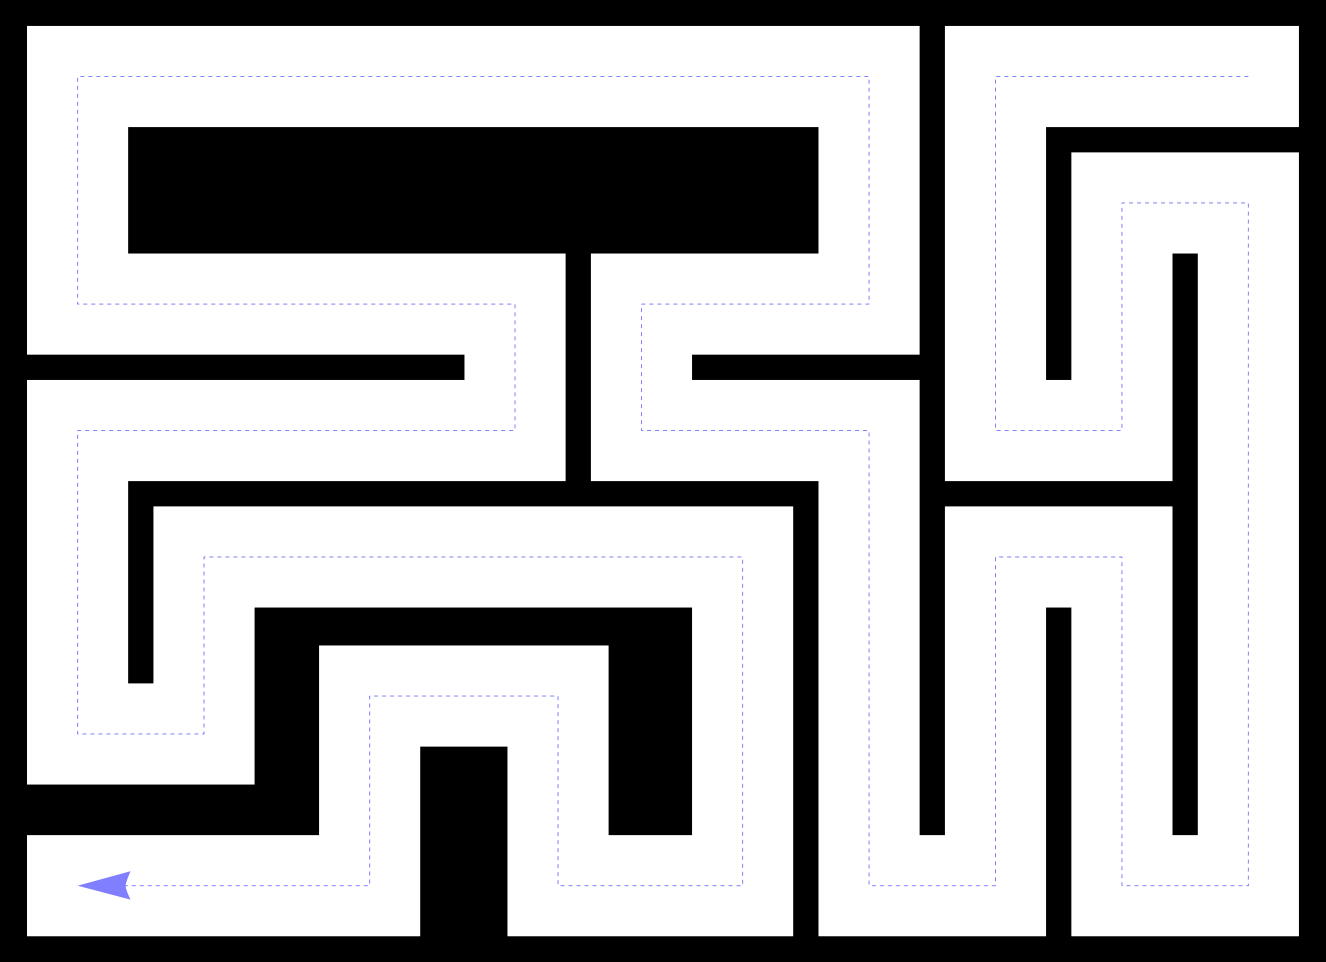
\includegraphics[width=.5\textwidth]{maze-representation.png}
\caption{Map of the maze.  Arrow indicates path direction.}
\label{fig:maze_with_path}
\end{figure}

\begin{figure}
\centering 
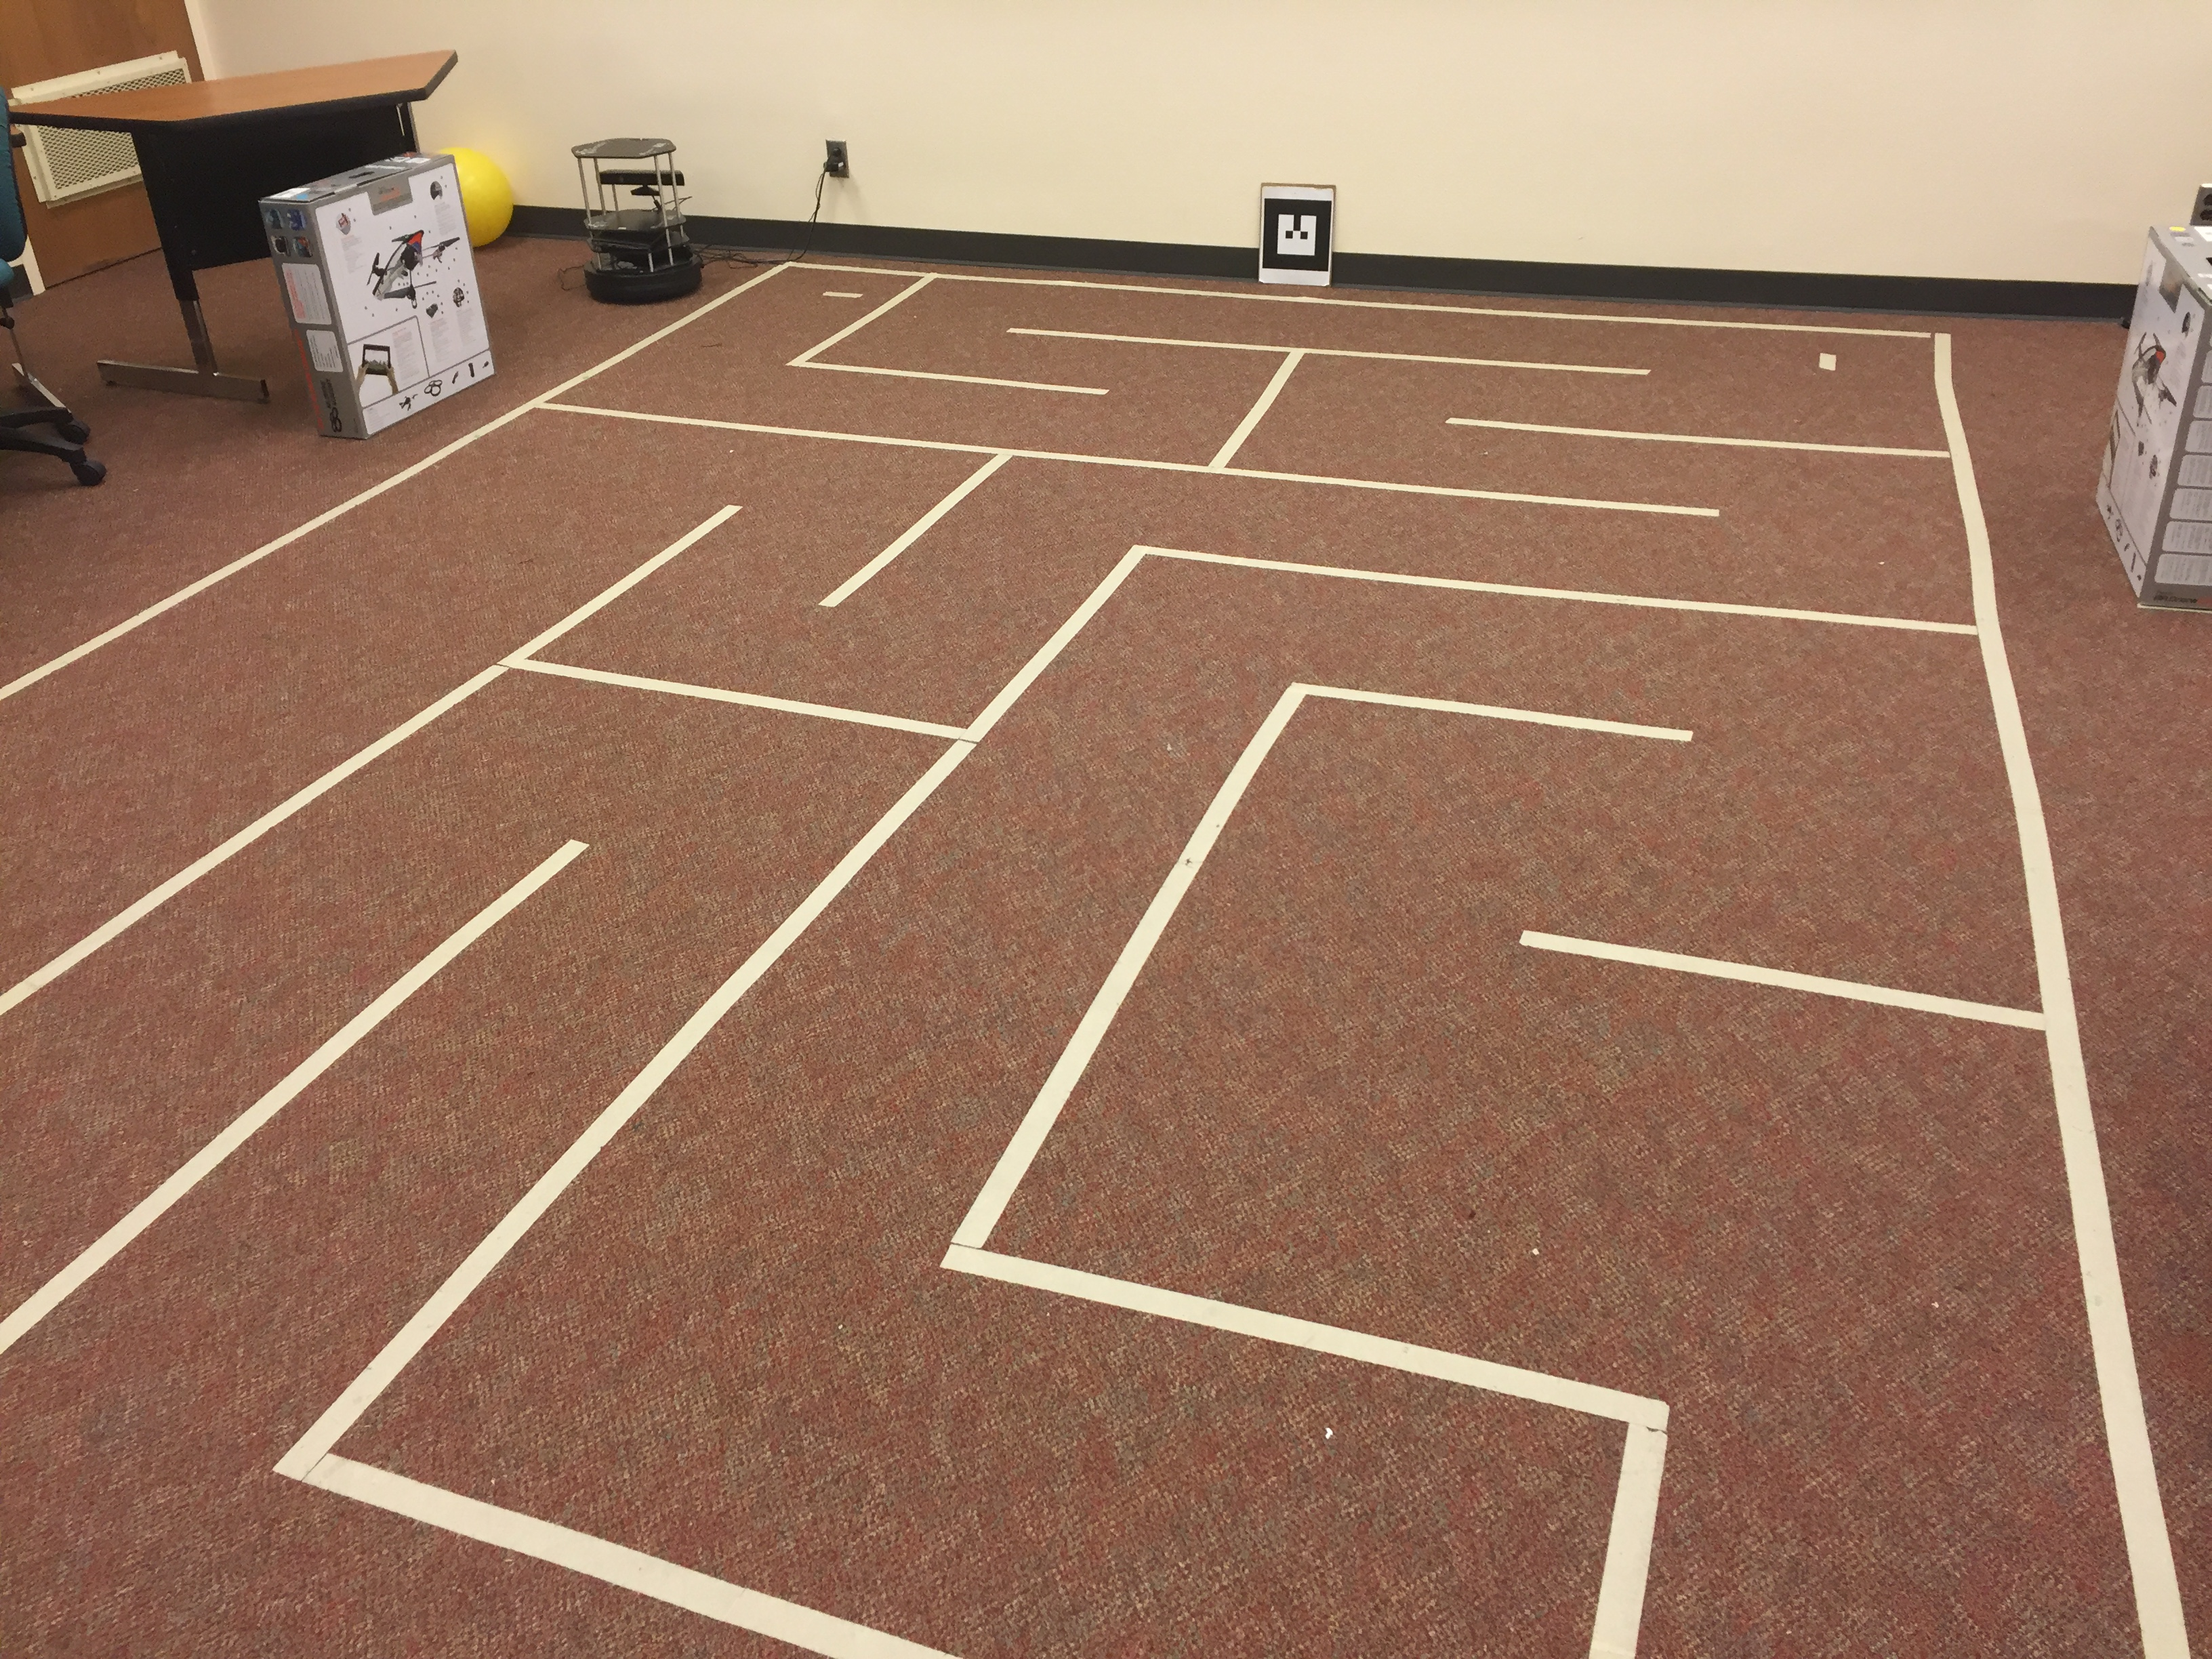
\includegraphics[width=.5\textwidth]{tape_map.JPG} 
\caption{The final map laid out on the lab floor.}
\label{fig:map_floor_img}
\end{figure}

As previously mentioned, the first step of our experimental design was
to identify a task simple enough for the robot to complete unaided,
yet complex enough to potentially benefit from human input. The
problem also need to be readily scalable to include additional
robots. This led us to select autonomous navigation through a maze
using Adaptive Monte Carlo Localization (AMCL). The maze
(Fig~\ref{fig:maze_with_path}) consisted of a single path with
multiple \text{90${}^{\circ}$} turns.  The final design, seen in
Fig~\ref{fig:map_floor_img}, consists of 32 waypoints and measures
$4.63m$ by $3.2m$. It is important to note that the maze traced out on
the floor serves only as a convenience for human operators and does
not serve as a navigation guide for the robot. In fact, the robot does
not treat the walls of the maze as physical obstacles, and will
happily pass through them if instructed to do so.

The robot's blithe ability to trundle through walls raises the
question of how the robot should differentiate between trustworthy and untrustworthy user input. For now, let's assume all the features that affect human cognitive stress are known and quantifiable and the robot's trust model is only concerned with a feature vector $ x \in R^{n \in \mathbb{N}} $ that contains all those metrics. For a known model, Maze Game, for example the trustworthy human instructions, in other words, the feature vector can be predefined. For example, the number of waypoints and there lengths are known.Therefore, in Maze Game, the feature vector $x$ contains the deviations from a trustworthy operations. Let's $\Delta m_j$ to be the $ j^{th} $ element of $x$. $\Delta m_j$ is the deviation that a human operator experiences or exposes in a task in $ j^{th} $ feature from a trustworthy human instruction. We will denote these deviations with a prefix $\Delta$. $\Delta m_j$ can be calculated as normalized real number within the range of 0 to 1 without any loss of generality. Calculation of $\Delta m_j$ may depend on another feature vector that has been generated by the previous human instructions, because intuitively, trustworthiness may depend on previous human instructions along with current instruction. We will show some examples of how these deviations can be calculated later in this section. We can define untrustworthiness $\mu $ of a vector $x$ as:
\begin{equation}
  \label{eq:general_untrust}
  \mu=\dfrac{\sum_{j} x_j}{\max (x_1,x_2, \ldots) - \min (x_1,x_2, \ldots)}
\end{equation}
As $\mu$ is normalized ($0\leq \mu \leq 1$), we can calculate trustworthiness $\tau$ of a human instruction by:
\begin{equation}
  \label{eq:general_trust}
  \tau=1 - \mu
\end{equation}

We can label the vectors with a $y = \{+1, -1\}$ using a decision function based on the trust value. The decision function decides whether an human assistance is trustworthy or not based on $\tau$ and a threshold $\theta$.

\[
y = 
\begin{cases}
+1, & \text{if } \tau\ge \theta\\
-1, & Otherwise\\
\end{cases}
\]

Now we have devised a generalised formulation for the sample feature vectors and corresponding labels for any known problem based on our Maze game. We can get input, label pairs as $(x, y)$ from a known task like Maze game. Then we can use an suitable machine learning tool to learn the trust model which will be then used in a new unknown  task. The essence of this experiment is that ideally, the learned model can be transferred to a new task and still the robot will be able to assess trustworthiness of human operator.
  
 In real world robot's trust model is concerned with limited number of features that are capitalized on the information gathered from both limited sensing capabilities and user feedback. For our Maze game,
these are: \textit{disparity}, \textit{percent damage} and \textit{goal arrival
  delay}:

\begin{description}
  \item[Disparity] is the Euclidean distance between the point the
    robot is expecting (located at the next turning point in the maze)
    and the point given by the user.
  \begin{equation}
  \label{eq:disparity}
  \Delta d^i=\sqrt{(x_{ideal}^i-x_{human}^i)^2+(y_{ideal}^i-y_{human}^i)^2}
  \end{equation}
  where $x_{ideal}^i$, $y_{ideal}^i$ and $x_{human}^i$, $y_{human}^i$ are the horizontal and vertical
  components of robot's position at the $i^{th}$ waypoint expected by the robot to reach and instruction given by the user respectively.

  \item[Health Damage Percentage] represents the cumulative "damage"
    the robot has sustained from colliding with the maze walls.
\begin{equation}
  \label{eq:health_calc} 
\Delta H^i = 
\begin{cases}
H, & \text{if } i = 0\\
\Delta H^{i-1}-randoms(0,\Delta H^{i-1}), & Otherwise\\
\end{cases}
\end{equation}
\begin{equation}
\label{eq:health_calc_norm}
h^i = \dfrac{\Delta H^i}{H}
s\end{equation}
  where $H$ is the initial health, $h_i$ the health upon reaching waypoint $i$ and function $random$ always returns a random number between to given parameters. Notice that $\Delta h^i$ is already normalized.
 
  \item[Time Delay] is the difference between when the robot would
    expect to reach a waypoint if it was navigating autonomously
    and the time taken when it is assisted by the human operator.
  \begin{equation}
  \label{eq:time_delay}
  \Delta t^i =t_{ideal}^i-t_{human}^i
  \end{equation}
  where $t_{ideal}^i$ is the time the robot would arrive waypoint $i$  navigating autonomously and $t_{human}^i$ is the actual arrival time when aided by the user.
\end{description}

We can take the normalized value for all the metrics defined as follows instead of Eq.~\ref{eq:disparity} and ~\ref{eq:time_delay}
respectively:

\begin{equation}
  \label{eq:disparity_norm}
  d^i = \dfrac{\Delta d^i}{\max(\Delta d^1,\Delta d^2, \ldots) - \min(\Delta d^1,\Delta d^2, \ldots)}
\end{equation}
 
\begin{equation}
  \label{eq:delay_calc_norm}
    d^i = \dfrac{\Delta t^i}{\max(\Delta t^1,\Delta t^2, \ldots) - \min(\Delta t^1,\Delta t^2, \ldots)}
\end{equation}

We can combine these metrics in such a way that a robot can evaluate
the trustworthiness of a user not only at a single instant, but also
obtain some notion of their overall trustworthiness.
Eq.~\ref{eq:mistrust} describes how well or badly a human operator is
actually performing while assisting a robot to navigate through the
maze game using ~\ref{eq:general_untrust}.
  \begin{equation}
  \label{eq:mistrust}
  \mu=\dfrac{d^i+h^i+t^i}{\max (d^i,h^i,t^i) - \min (d^i,h^i,t^i)}
  \end{equation}

Eq.~\ref{eq:mistrust} express our idea about the untrustworthiness of
human operator because all three terms on the right hand side of the
equation negatively affect the effectiveness of the maze navigation
task. For example, we want the robot to reach the intended key point
as closely as possible. Thus, an absolute trustworthy value of
disparity is zero. It is also easy to see that disparity is always
non-negative.  On the other hand, delay can be negative or positive. A
positive delay negatively affects the effectiveness of the task;
ideally the robot should reach its goals more quickly with human
assistance than without. The last term, damage, is calculated in a
different way than the previous two terms. The health metric is
quantifiable but is fairly arbitrary and abstract compared to the
other two metrics. The robot is assigned an initial $h_0$ value, and
whenever the robot makes contact with a wall of the maze, the health
value is decreased by a randomly-varying amount.  The damage metric,
then, denotes how consistently the robot was able to follow human
assistance under a collision constraint.

Eq.~\ref{eq:mistrust} thus provides a value that tells us how much
untrustworthy a human assistant was. However, the terms that
constitute the formula are not numerically in the same scale.  Thus
they may not provide us with good intuition about
untrustworthiness. Moreover, we are interested in calculating the
trustworthiness of the human operator, rather than the
untrustworthiness. Although these values are complimentary, the former
version is more intuitive.  We therefore normalize the metrics so that
trustworthiness falls in the range $0$ to $1$.  


One of the concerns with the normalization of $d, h, \Delta t$ and
$\tau $ is the potential loss of of information that could lead to
misclassification. We have plotted the histogram distribution of all
the metrics.  Fig~\ref{fig:hist_norm} demonstrates that the
distribution of the data remains largely intact.

\begin{figure}
\centering
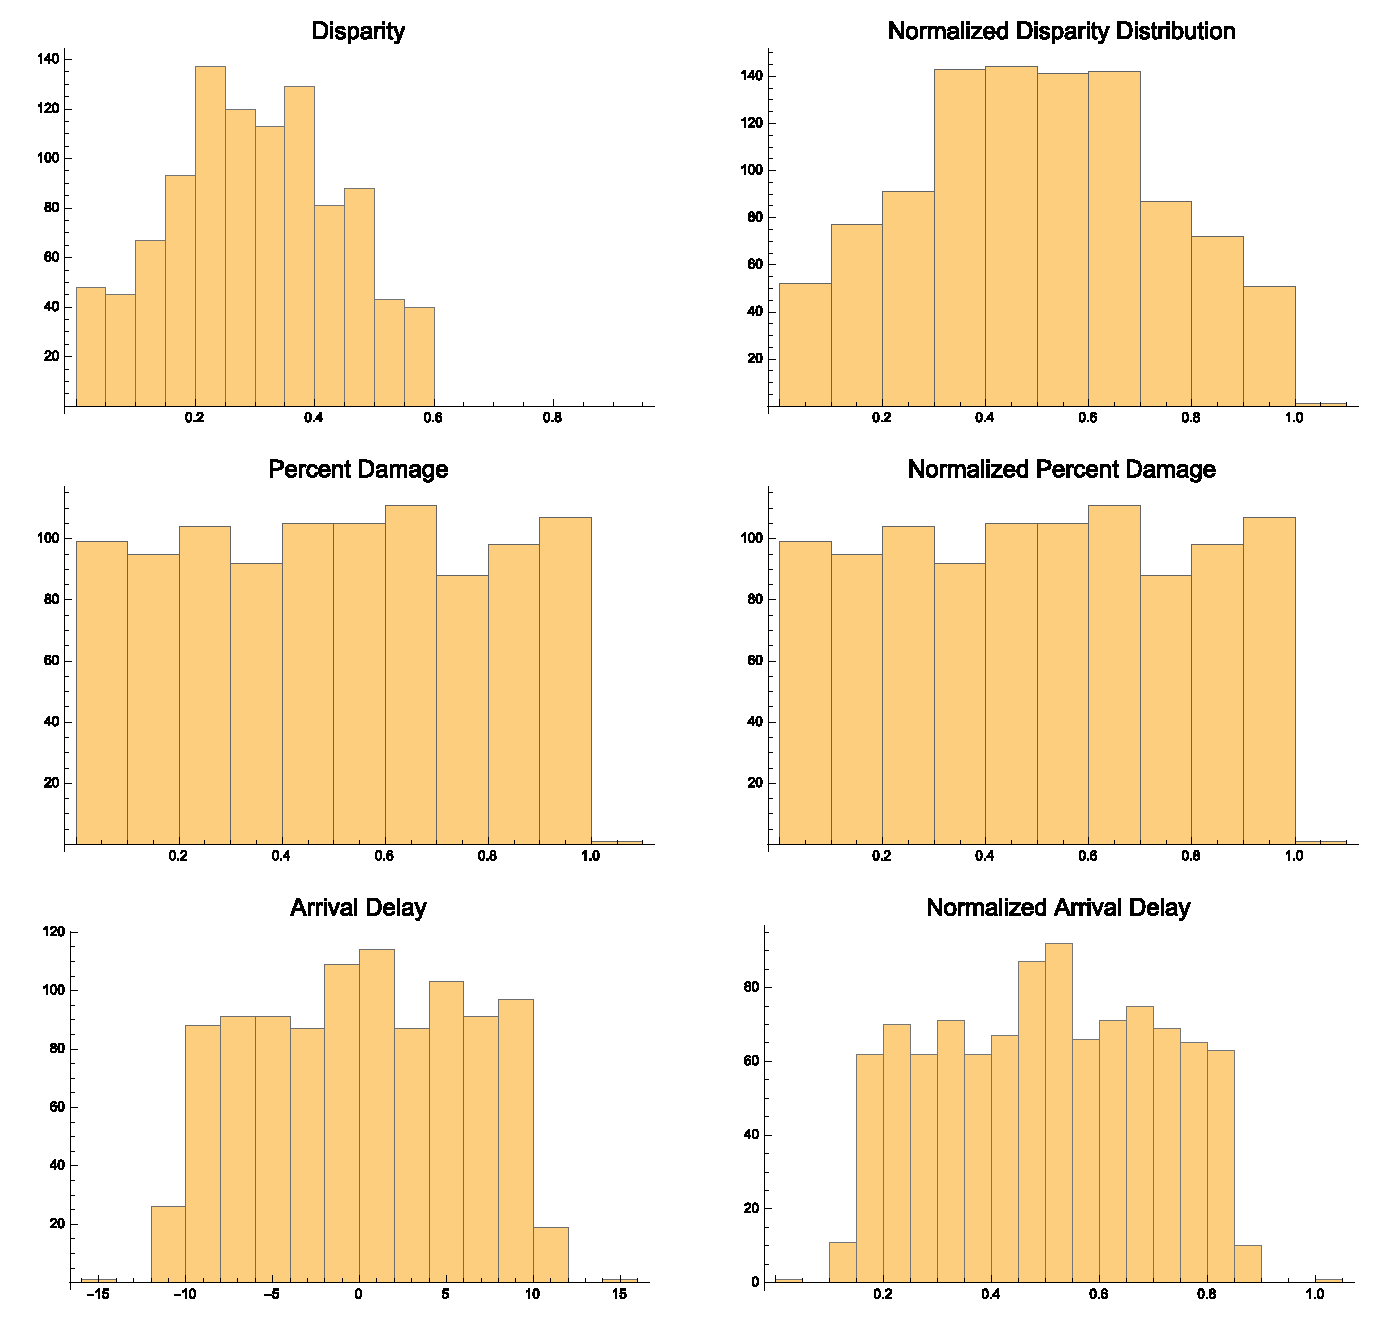
\includegraphics[width=.5\textwidth]{histograms.eps} 
\caption{Comparison between histograms of $d, h, \Delta t$ and $\tau$
  before and after normalization.}
\label{fig:hist_norm}
\end{figure}
 
It is worth noting that in this experiment the robot can only move
forward to each successive point on the path. Together, these points
form an indexed list. An index is incremented by control program for
the experiment if it reaches the next key point. Therefore, helpful
assistance from the human operator will provide the next key point in
the maze. A poor performance by a cognitively-stressed human operator
will be punished by several metrics. For example, if a human operator
points the robot at a goal which is across the wall of the maze, then
the robot will hit the wall, damaging the robot's health and
negatively affecting the trustworthiness.  Similarly, a human operator
who is unable to pay close attention to the robot interaction will
fail to provide timely instructions to the robot, and the robot will
therefore take more time to reach its goal.  Again, this results in a
poor delay score and will affect the trustworthiness of the human
operator as expected. Lastly, if the operator instructs the robot to
make for an unknown or distant goal location, it will affect the
trustworthiness by contributing to disparity metric.  From the above
discussion it becomes clear that our chosen metrics should be
effective in determining the trustworthiness of the human operator. We
will formally show the evidence of our claim in the next sections.

\subsection{Maze Game and Training Results}
Now we will show that Eq.~\ref{eq:trust} indeed reflects the
trustworthiness of humans correctly, based on the described metrics,
and we will demonstrate that the robot has learned a model that can
predict the trustworthiness of human operator in a different context.
Six test subjects performed runs of the maze game, resulting in
approximately $1000$ instances of trustworthiness data defined by
Eq.~\ref{eq:trust}.

\begin{figure}
\centering
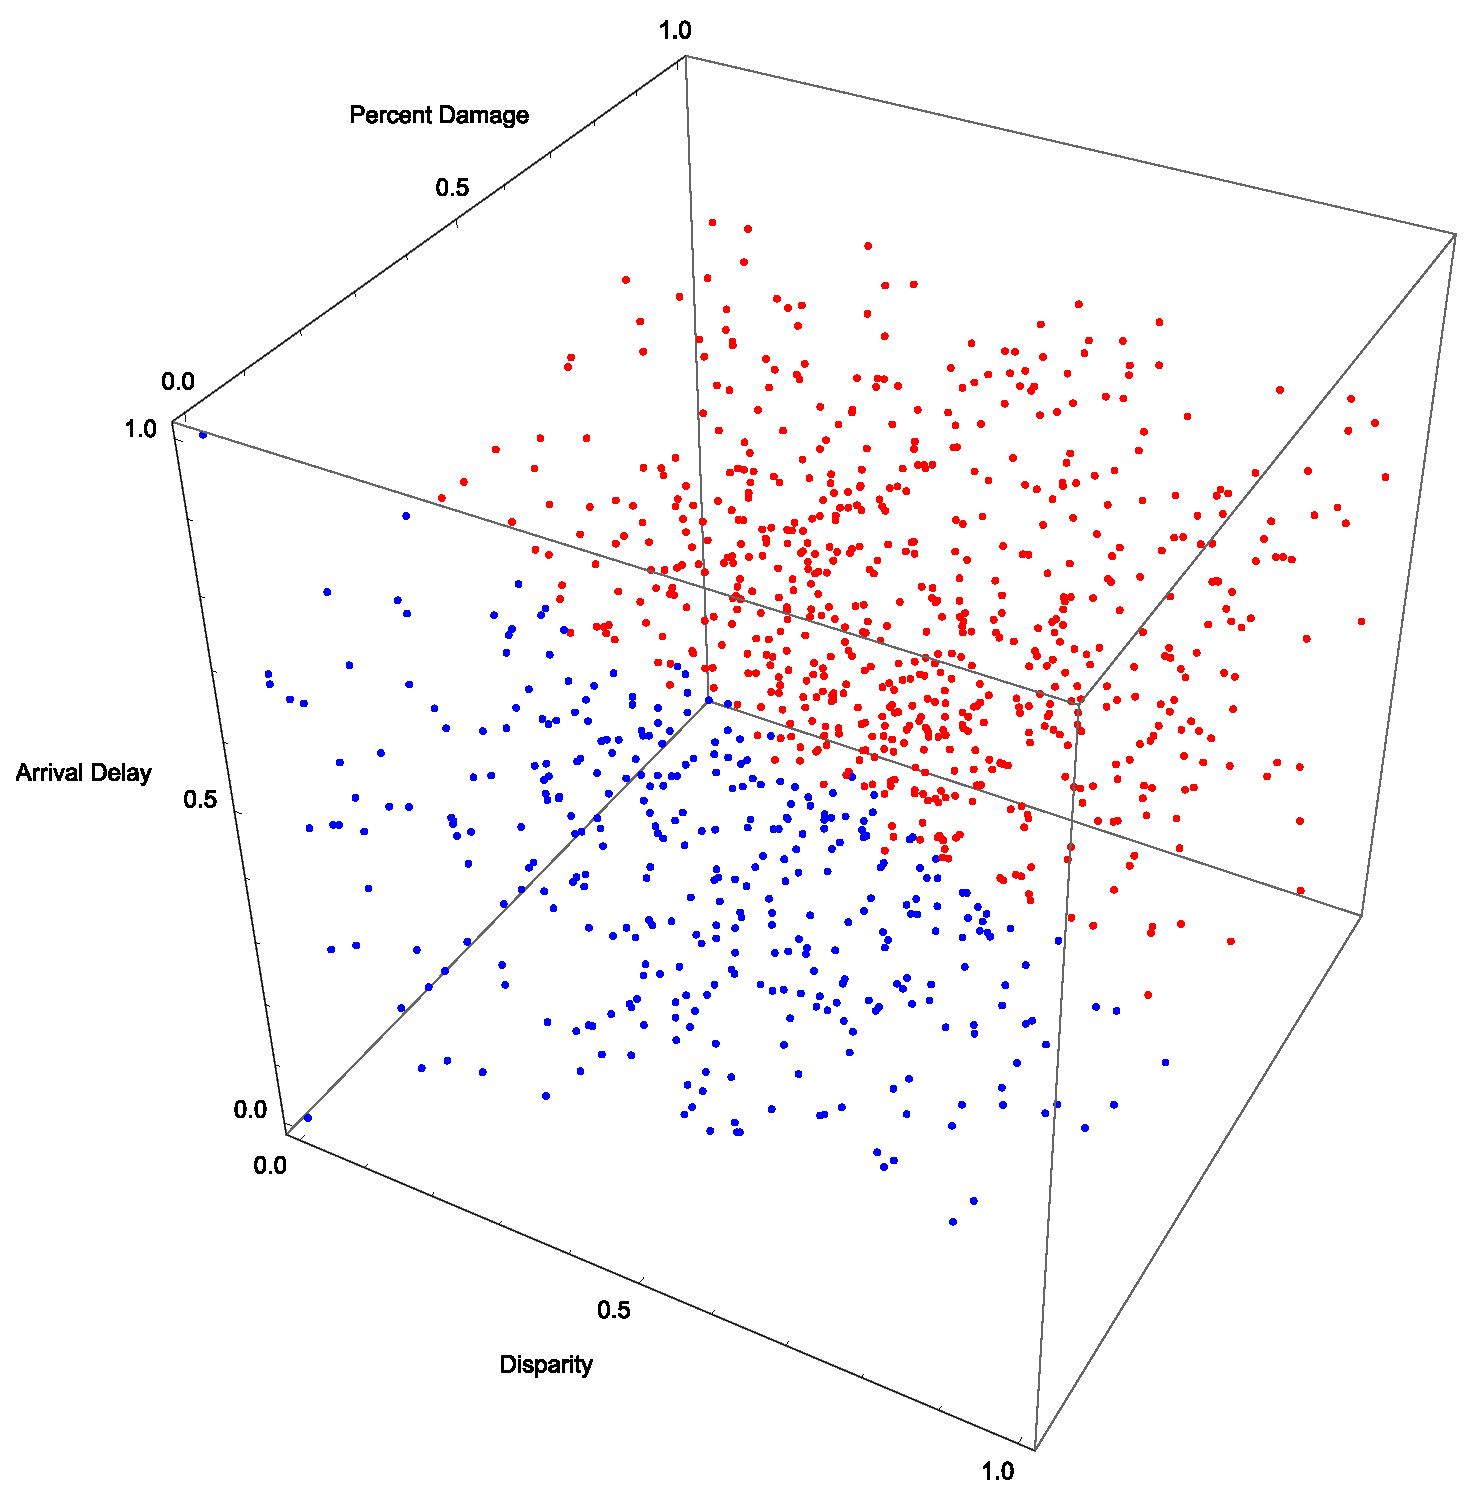
\includegraphics[width=.5\textwidth]{4d-plot.eps}
\caption{Disparity, Damage, Delay vs. Trustworthiness.  The robot has
  adjudicated red dots as untrustworthy and blue dots as trustworthy.}
\label{fig:data_maze_game}
\end{figure}

Fig.~\ref{fig:data_maze_game} shows a four-dimensional scatter plot
that shows the robot's judgment of trustworthiness with respect to the
humans' performance metrics.  Because the robot understands the maze
game and the details of the performance metrics, it is able to
generate the training data labels for a supervised model learning
task.  We have used the Orange data mining
API\footnote{http://orange.biolab.si} for this purpose.  The human
performance metrics and the robot's self-generated classification are
used to train a Support Vector Machine (SVM) classifier.  SVMs are
able to capture a classifier hyperplane even in high-dimensional
spaces. SVMs have been used to learn enormous classifiers in very
complex feature spaces including cancer cell detection and spam email
classification \cite{guyon2002gene, drucker1999support}.  The maze
game classifier is only a two-dimensional plane in three-dimensional
feature space (see Fig.~\ref{fig:data_maze_game}), so an SVM should be
able to learn a classifier from our experimental data effortlessly,
and the approach should scale to much more complex feature spaces.
Here, we have two classes $y\in\{-1,1\} $ which denotes whether to
trust or not to trust the operator respectively.  The training data is
specified as $x_i = [d_i, h_i, \Delta t_i]^T$. Our input for the
classifier is $(y_1,x_1), \ldots,(y_N,x_N)$. The SVM generates an
optimized $w$ that identifies the hyperplane to classify test data by
minimizing the following function:
\begin{equation*}
\begin{array}{ccc}
\frac{1}{2}w^{T}w + C\sum _{i=1}^N \xi _i \\
\text{with the following constraints,} \\
y_{i} = (w^{T}x_{i} + b)\geq 1-\xi_{i} \text{and} \xi_{i}\geq 0, i=1,...,N
\end{array}
\end{equation*}
Here $C $ and $b $ are constants. $\xi $ denotes the non-separability
of the input data.

The classifier was trained using two different methods;
cross-validation and leave-one-out.  Both of the data sampling methods
provided good classification accuracy. In the cross-validation method
we sampled 70\% of the data from the maze game to use as training
data, which resulted in a 95\% accuracy in the classification on the
test data sample. In the leave-one-out method, all instances except
one are selected for training the classifier. After that, the test
data set is classified using the learned model. All of the instances
are selected at least once as test data. The total accuracy of the
classification is calculated by counting the percentage of data that
has been selected and classified correctly against the total data
set. This method also resulted in 95\% of the data being correctly
classified.
%The result of the classifier on the test data using different sampling size using cross validation method in the first experiment is shown in Table~\ref{tab:acc_maze_game}

%\begin{table}
%\centering
%\caption{Accuracy of the classifier in the maze game experiment.}
%\label{tab:acc_maze}
%\begin{tabular}{|c|c|} \hline
%Training Size & Accuracy of classification\\ \hline
%45\% & 95\% \\ \hline
%50\% & 95\% \\ \hline
%55\% & 95\% \\
%\hline\end{tabular}
%\end{table}

Another way to observe the confidence of the classifier is a confusion
matrix. The confusion matrix for the classifier using cross-validation
and the leave-one-out method is shown in
Table~\ref{fig:conf_matrix}. The diagonal elements of the classifier
show how accurately the classifier has worked on a given data set. The
table shows that 131 of 133 human assistance data points were
correctly classified as untrustworthy, while all 68 trustworthy
data points were correctly classified.

\begin{figure}
\centering
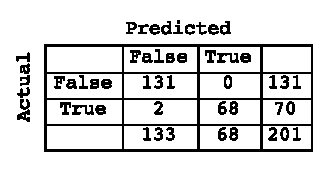
\includegraphics[width=.3\textwidth]{confusion-matrix.eps}
\caption{Classifier confusion matrix.}
\label{fig:conf_matrix}
\end{figure}

%\begin{table}
%        \caption{Confusion matrix of the classification using cross validation method.}
%        \label{tab:conf_cross}
%        \begin{tabular}{|p{1.5cm}|p{1.5cm}|p{1.5cm}|p{1.5cm}|}
%            \cline{1-4}
%            \multicolumn{2}{|p{1.5cm}|}{} & \multicolumn{2}{|c|}{Prediction} \\
%            \cline{3-4}
%            \multicolumn{2}{|p{1.5cm}|}{} & True & False\\
%            \cline{1-4}
%            \multirow{2}{*}{Actual} & True & 72 & 10\\\cline{2-4} & False & 10 & 72\\ \hline
%        \end{tabular}
%    \end{table}
    
%\begin{table}
%    \caption{Confusion matrix of the classification using leave one out method.}
%    \label{fig:conf_matrix}
%    \begin{tabular}{|p{1.5cm}|p{1.5cm}|p{1.5cm}|p{1.5cm}|}
%        \cline{1-4}
%        \multicolumn{2}{|p{1.5cm}|}{} & \multicolumn{2}{|c|}{Prediction} \\
%        \cline{3-4}
%        \multicolumn{2}{|p{1.5cm}|}{} & True & False\\
%        \cline{1-4}
%        \multirow{2}{*}{Actual} & True & 72 & 10\\\cline{2-4} & False & 10 & 72\\ \hline
%    \end{tabular}
%\end{table}
     
\section{Coin Game Experiment}

The second phase of the project involves a variation on the first
experiment dubbed the Coin Game. It uses many of the same principles
introduced in the Maze Game, such as the same map, but also places new
constraints on both the user and the robot. For example, in this
experiment the goal is not defined by the human operator; rather the
goals appear randomly in the maze. We call these random goals "coins",
with the understanding that the point of the game is to send the robot
to the coin locations in order to collect them. Unlike in the previous
experiment, where the robot navigated the maze in linear fashion from
start to finish, the goals or coins may pop up in any location in the
maze, either ahead of or behind the robot. As the goal is generated
randomly and not under the control of the human operator, it puts more
cognitive stress on the operator than the previous experiment, as we
will see in the experimental results. Another aspect of cognitive
stress for the human operator is that in this experiment, the goal is
not represented in the real world; rather the goals are shown on the
control interface's computer screen as colored circles denoting the
coins. Coins can pop up between any two key points. The map of this
experiment has been shown in Fig.\ref{fig:coin_map}. Matching the
location in the map and real world may pose some additional challenge
on human operator. In short, although the second experiment has a very
similar setup to the first experiment, it is indeed a different
problem. But it is a suitable problem to test our learned model
because many of the metrics here have similar implication as they had
in the previous experiment.

\begin{figure}  
\centering
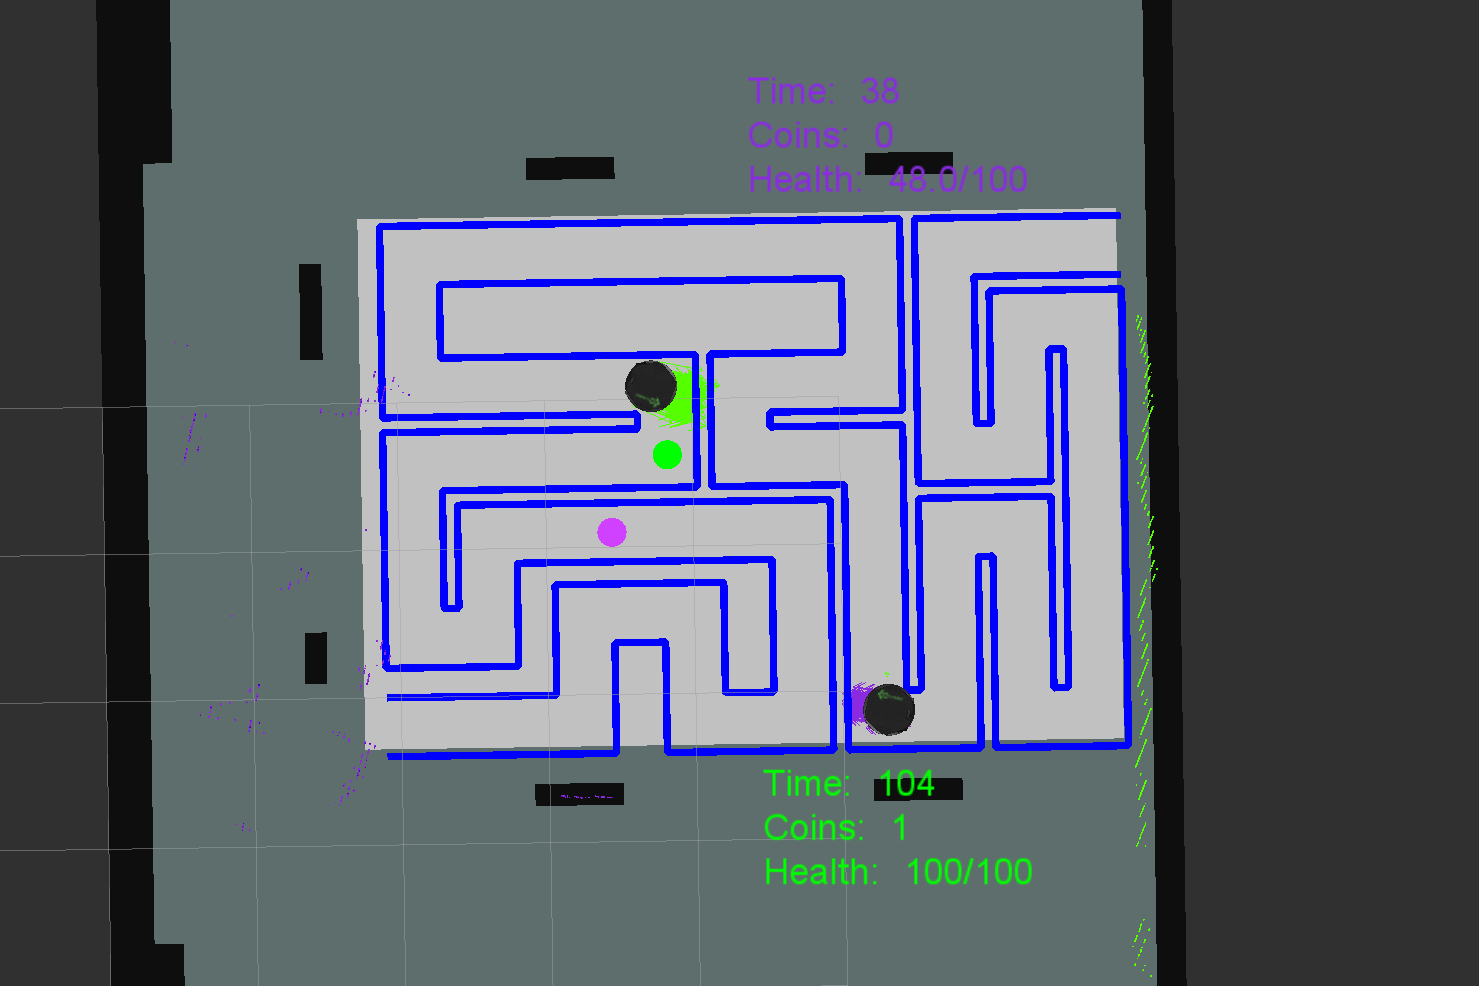
\includegraphics[width=.5\textwidth]{coin_game_rviz.png}
\caption{Maze map of the Coin Game experiment with coin goals.}
\label{fig:coin_map}
\end{figure}

The coin game is a very simple game. The human operator points the
mouse to a location the map. As the goal is random, the human operator
must now switch between robots frequently, in order to marshal the
various robots toward their coin goals. Research
\cite{olsen2003metrics} has shown that this switching time can affect
the effectiveness of a task performed by the human robot team. Thus
the second experiment is more challenging in terms of cognitive
stress.  The task sets a two-minute timer for the human operator and
also sets a maximum 5 coin collection limitation. Either condition
satisfies the end of the game. Every time the robot collects a coin
the timer is shortened by 12 seconds to put more cognitive stress on
human operator.

Even though all the metrics used in the first experiment have a
similar implication in this experiment, the robot cannot calculate
them as effectively, because it does not have independent knowledge of
goal locations beyond the physical characteristics of the maze
environment. For example, the ideal arrival time to a key point can be
calculated by determining the path segments from the robot's current
position and then adding the corresponding required ideal time, but
whether the key point is appropriate or not is beyond the robot's
knowledge.  The learned classifier will classify the the human
assistance based on the disparity, damage and time delay it produces,
even though these figures are calculated based on invalid assumptions
about the nature of the game.  Nevertheless, the robot feeds these
metrics into the classifier that was learned in the maze game to
produce a ``trustworthy'' or ``untrustworthy'' output.  It has no
access to a formula to make this determination, since the maze game
formula is specific to that well-understood problem.

%We have set two scenarios in this experiment. The first scenario, is the single human operator one or more robots team. In this scenario only one human operator was allowed to assist the human-robot team. We have set a timer for the human operator as 2 minutes and also set maximum 5 coin collection limit. Either condition satisfies the end of the game. Every time the robot collects a coin the timer is shortened by 12 seconds to put more cognitive stress on human operator. In the second scenario, multiple one or more robots were teamed up with two human operators. The initial timer was set to 1 minute and a maximum of ten coins were allowed to collect. Either condition satisfied he end of the game.

\subsection{Coin Game Results}

Analysis of the results from the coin game experiment are in agreement
with the original hypothesis. In general, the robot correctly predicts
the cognitive load that its operator was under in every
scenario. These findings can be seen in Fig~\ref{fig:final-results}.
Here, the $x$ axis denotes an increase in task complexity over time;
the user must issue an increasing number of commands and collect coins
in an increasingly short duration. It is critical for interpreting the
information in \ref{fig:final-results} to note that while the robot's
cognitive load evaluation and the scoring technique for quantifying
self-reported user stress both produce a result between zero and one
\textit{their magnitudes are not directly comparable}.  The points at
which stress was identified, and the shape of the curves, however, are
appropriate to compare.  Whenever cognitive stress occurs or changes,
the robot is able to recognize this increase for most cases in the
tested scenarios, and the robot's evaluation agrees with self-reported
user stress.  In the context of this paper, it also supports the
original hypothesis: robots can are able to reliably assess the
cognitive strain their human partners are under, even in contexts
where the actual tasks they are being asked to perform are opaque to
the robot.

%Six people who participated in first experiment also participated in
%the second experiment. We have found that the learned model of
%classifier was able to understand good and bad assistance very
%efficiently. We did not allow the robot to change its behavior based
%on the trustworthiness; it is just keeping a log of which of the
%assistance came from the human operator were trustworthy and which
%were not. While running the second experiment we manually kept a log
%to indicate which particular human assistance were seemed to be
%trustworthy in the naked eye. After the experiment we collected the
%log from the robot and then compared with our human judged
%interpretation of trustworthiness. We have found that the 95\% and
%97\% of robots prediction matches with the two human
%interpretations. This is a very promising result to support our
%hypothesis in Eq.~\ref{eq:trust_norm}. The result also showed decrease
%in trustworthiness as the complexity of the task increases. The result
%on matching classification on different level of complexities are
%shown in the following Fig\ref{fig:final-results}:

\begin{figure}  
\centering

\includegraphics[width=.25\textwidth]{final-legend.eps}
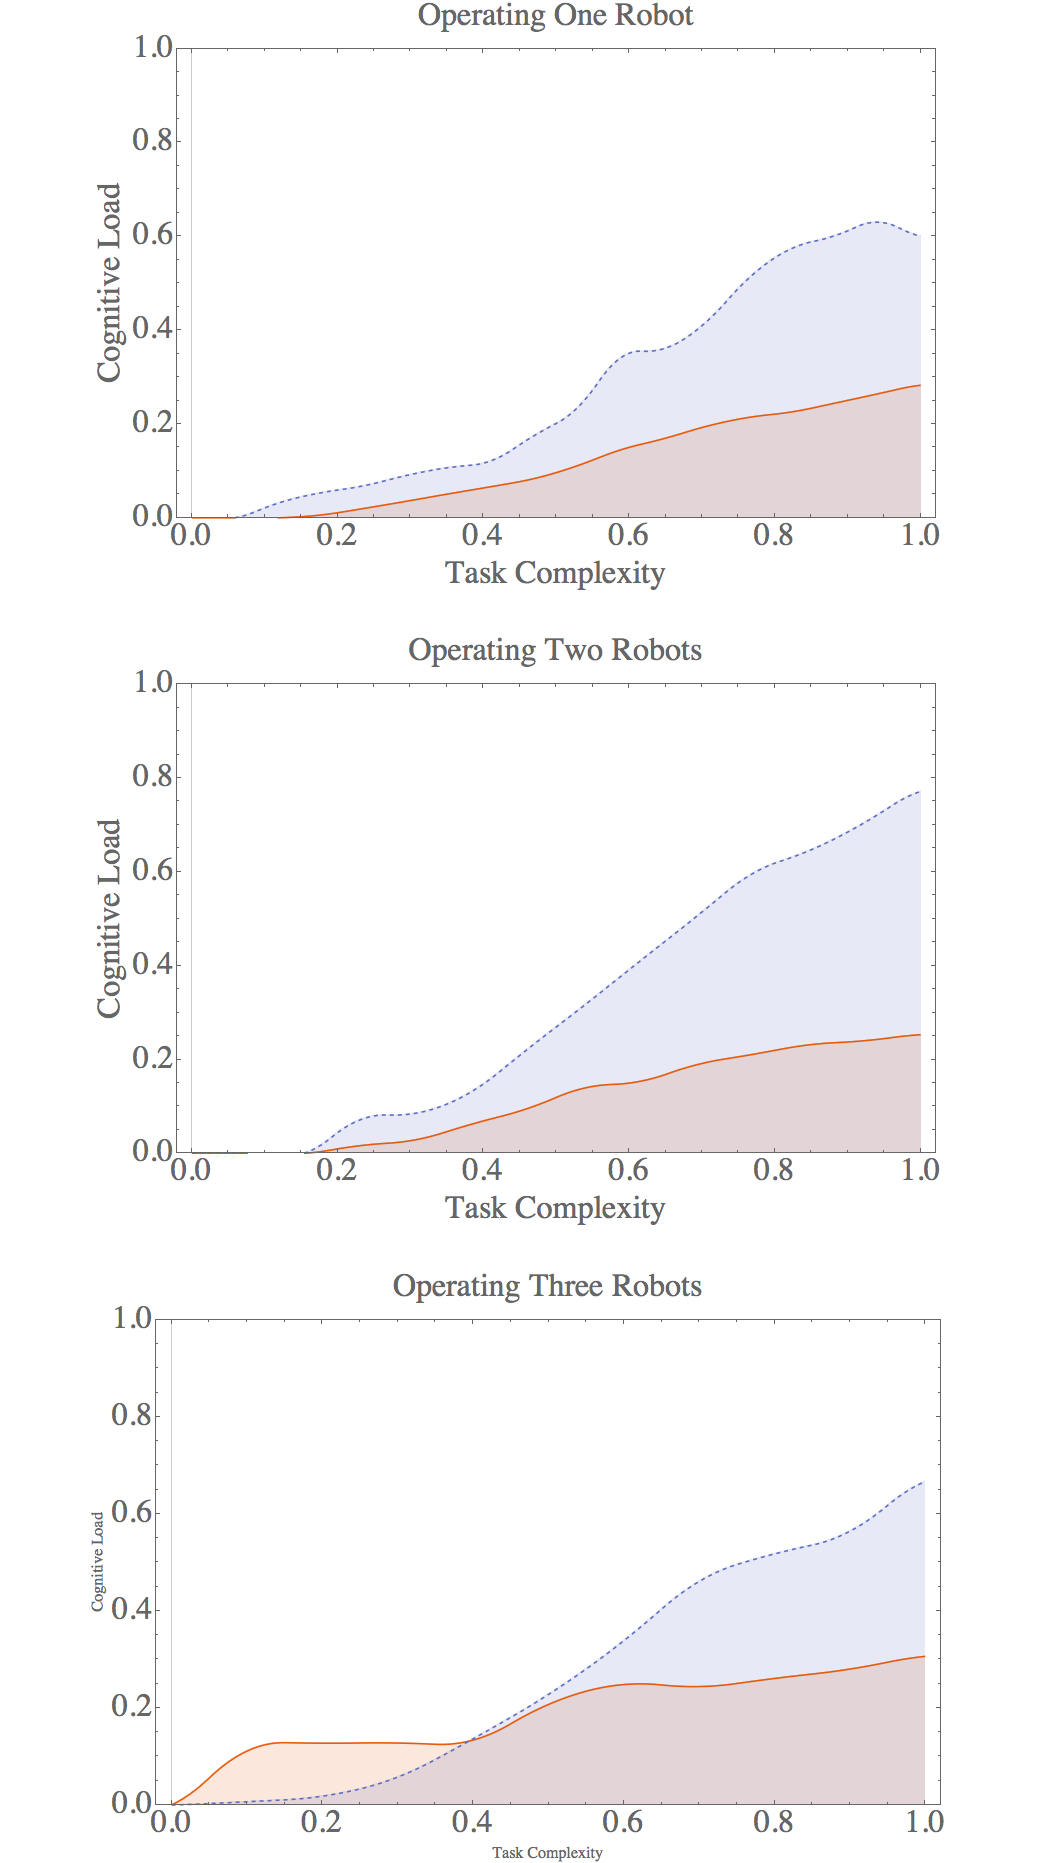
\includegraphics[width=.5\textwidth]{final-results.png}
\caption{Cognitive load of human operator in Coin Game experiments with differing numbers of robots and steadily increasing task complexity.}
\label{fig:final-results}
\end{figure}

\section{Conclusions}

The field of human-robot interaction began by investigating how robots
can be designed so that they are comfortable, predictable and
understandable to their human partners.  Our work investigates an
aspect of the other side of that equation: what can robots understand
about us?  Robots that are capable of understanding the stress or
strain their operator is experiencing are vital to safe and efficient
teamwork in complex scenarios where the proper level of autonomy and
interaction is fluid.  Vital communication cues are embedded in the
way we behave in particular circumstances, and these implicit
indicators do not have to be lost on our robots.  Our work's
contribution is to demonstrate a quantitative, learnable,
generalizable model that allows a robot to determine that a user is
behaving in an untrustworthy fashion, even when the robot cannot
independently assess the instructions it is being given.  Another
important finding is that the threshold beyond which cognitive stress
produces untrustworthy human assistance may vary from task to task.
Nevertheless, general metrics can transfer from problem to problem and
still produce meaningful evaluations.  In the future, we plan to
extend this research into complex heterogenous teams of humans and
robots performing real-world tasks.

Every day humans interact with more and more technologies that require
us to decide whether or not to trust them; robots should be making
similar determinations about us.

%Our research has a profound implication on the way used to look into
%human robot team. One vital contribution of this paper is that it
%shows that trustworthiness of human operator in human-robot team can
%be quantified and learned using useful metrics. We can define it by
%the term transfer effectiveness of human operator. Besides, defining
%this novice terminology we have also achieved significant evidence to
%show transfer effectiveness is possible across multiple problem
%domain. We have done two experiments on human-robot team to assess
%cognitive capacity of human assistance. For our a particular problem
%of maze game, metrics like our disparity, arrival time delay and
%damage considered as vital metrics in determining the
%trustworthiness. We have shown that the learned model also implies on
%Coin Game problem which our second experiment. Although, built on
%similar set-up, the second experiment was different in many ways from
%the first. We showed that, although they are different the
%trustworthiness classifier model can be transferred to this new domain
%of problem effectively. From this experimental result we try to say
%that for if several human-robot team problems have metrics those have
%common implications, may help us to learn the nature of of human
%assistance cognitive behaviour for those problems. It may also help us
%to infer the human cognitive stress limitation in another problem. In
%other words, our research showed that cognitive capacity of human
%assistant is transferable.


\section{Acknowledgments}
Acknowledgments are redacted for anonymity during the review process.

%We would like to thank Robotic Cognition Laboratory of Computer Science Department of Oklahoma State University for facilitating this project. We would also like to thank all the people who participated in the project as human operator voluntarily.

\bibliographystyle{abbrv}
%\bibliographystyle{acmlarge}
\bibliography{sigproc-2}

\end{document}
